\documentclass[twocolumn, fontsize=10pt]{article}
\usepackage[margin=0.70in]{geometry}
\usepackage{lipsum,mwe,abstract}
\usepackage[english]{babel} 
\usepackage{fancyhdr} % Custom headers and footers
\pagestyle{fancyplain} % Makes all pages in the document conform to the custom headers and footers
\fancyhead{} 
\fancyfoot[C]{\thepage} % Page numbering for right footer
\setlength\parindent{0pt} 
\usepackage{amsmath,amsfonts,amsthm} % Math packages
\usepackage{wrapfig}
\usepackage{graphicx}
\usepackage{float}
\usepackage{subcaption}
\usepackage{comment}
\usepackage{enumitem}
\usepackage{makeidx}
\makeindex
\usepackage{cuted}
\usepackage{sectsty} % Allows customizing section commands
\usepackage{xcolor} % For colored text
\usepackage{hyperref} % Package for links
\hypersetup{
    colorlinks=true,
    linkcolor=blue,
    filecolor=magenta,      
    urlcolor=blue,
    }
\allsectionsfont{\normalfont \normalsize \scshape} % Section names in small caps and normal fonts

\addto\captionsenglish{\renewcommand{\contentsname}{Índice}}

\renewenvironment{abstract} % Change how the abstract look to remove margins
 {\small
  \begin{center}
  \bfseries Resumen \vspace{-.5em}\vspace{0pt}
  \end{center}
  \list{}{%
    \setlength{\leftmargin}{0mm}
    \setlength{\rightmargin}{\leftmargin}%
  }
  \item\relax}
 {\endlist}

 \newenvironment{englishabstract} % Abstract en inglés
 {\small
  \begin{center}
  \bfseries Abstract \vspace{-.5em}\vspace{0pt}
  \end{center}
  \list{}{%
    \setlength{\leftmargin}{0mm}
    \setlength{\rightmargin}{\leftmargin}%
  }
  \item\relax}
 {\endlist}
 
\makeatletter
\renewcommand{\maketitle}{\bgroup\setlength{\parindent}{0pt} % Change how the title looks like
\begin{flushleft}
  \begin{center}
    {\color{black} \Large Facultad de Matemática y Computación. Universidad de La Habana. \\
    \color{black} Inteligencia Artificial y Simulación. \\ \vspace{10pt}}
    \href{https://github.com/DanielMPMatCom/AI-Simulation-Project-2024.git}{Repositorio del Proyecto en GitHub} % Add GitHub link here
    \vspace{10pt}
  \end{center}
  \textbf{\@title}
  \@author \\ 
  \@date
\end{flushleft}\egroup
}
\makeatother

%% ------------------------------------------------------------------- 

\title{

\Large Simulación de un Sistema Eléctrico basado en Plantas Termoeléctricas.  \\
[10pt] 
}
\date{\today}
\author{Daniel Machado Pérez - daniel.machado.0206@gmail.com \\
Daniel Toledo Martínez - daniel020126@gmail.com \\
Osvaldo R. Moreno Prieto - osvaldo020213@gmail.com}

\begin{document}

\twocolumn[ \maketitle ]



% --------------- ABSTRACT
\begin{abstract}
    Este proyecto se centra en la simulación de un sistema de plantas termoeléctricas
    que abastecen de energía a varios circuitos distribuidos en una región geográfica.
    Se implementa un generador de un mapa del sistema, ubicando circuitos, termoeléctricas
    y una línea principal a la que se conectan todos los componentes y por la que pasa toda
    la energía producida. Cada termoeléctrica cuenta con varias partes o piezas que garantizan
    su funcionamiento, y un agente planificador con arquitectura BDI que se encarga de tomar decisiones
    sobre el régimen de mantenimientos y reparaciones a las piezas. Cada circuito consta de uno o más bloques 
    que lo dividen y reciben electricidad por separado. Por último existe un agente superior que simula
    al Jefe de la Empresa Eléctrica y toma decisiones con respecto a la distribución óptima de electricidad, 
    también con arquitectura BDI. Para garantizar la efectividad de las decisiones se utiliazn
    componentes de Búsqueda, Conocimiento y Procesamiento de Lenguaje Natural.

\end{abstract}

\begin{englishabstract}
  This project focuses on the simulation of a system of thermoelectric plants that supply energy to various circuits distributed across a geographical region. A system map generator is implemented, placing circuits, thermoelectric plants, and a main power line connecting all components, through which all produced energy flows. Each thermoelectric plant consists of several parts that ensure its proper functioning, and a BDI (Belief-Desire-Intention) architecture planning agent is responsible for making decisions regarding the maintenance and repair schedule of these parts. Each circuit is divided into one or more blocks, which receive electricity separately. Additionally, there is a higher-level agent simulating the Chief of the Electric Company, who makes decisions regarding the optimal distribution of electricity, also based on a BDI architecture. To ensure the effectiveness of decision-making, components from the fields of Search, Knowledge Representation, and Natural Language Processing, within Artificial Intelligence, are utilized.
\end{englishabstract}

\rule{\linewidth}{0.5pt}

% --------------- KEYWORDS
\noindent \textbf{Palabras Clave}: Termoeléctrica, Circuito, Bloque, Caldera, Generador, 
Turbina de vapor, Serpentines, Agente, BDI, Belief, Desire, Intention, Algoritmo Genético (GA), 
Lógica Difusa, Modelo Extenso de Lenguaje (LLM)



% --------------- MAIN CONTENT

\tableofcontents

\section{Introducción}

En esta sección estaremos definiendo el problema en cuestión, 
sus componentes (que serán abordadas a detalle más adelante),
los objetivos planteados y algunas cuestiones técnicas que
forman parte del marco teórico sobre el que se sustenta la investigación.

\subsection{Descripción del Proyecto}

El \textbf{Sistema Eléctrico} que se consideró consta de un conjunto de \textbf{Plantas Termoeléctricas}
situadas relativamente cercanas a un conjunto de circuitos distribuidos en un mapa 2D.
Se asume que cada termoeléctrica consta de 4 tipos de piezas principales:
\textbf{Calderas}, \textbf{Turbina de Vapor}, \textbf{Serpentines}, \textbf{Generador} \cite{parts}.
En este proyecto se decidió abstraerse de la función que cumple cada una de estas piezas
en una verdadera Planta Termoeléctrica. En cambio se otorgó relevancia a la implicación de
una rotura de cada una de ellas en el rendimiento de la termoeléctrica. Se asumió que una planta
 puede tener una o más calderas, y que la generación de la planta está dividida en cada una de sus calderas,
 es decir, al romperse una caldera se pierde la generación que corresponde a la capacidad máxima entre el total
 de calderas. Eso quiere decir que si dejan de funcionar todas las calderas al mismo tiempo la planta no producirá energía.
 En cuanto a las demás partes, cada planta posee una sola de cada una de ellas y su rotura implica la salida de circulación
 de la termoeléctrica del sistema eléctrico. Cada termoeléctrica tendrá una generación máxima, una ubicación en el mapa,
 una planilla del costo de suministrar energía a cada circuito, una energía almacenada y un \textbf{Agente} planificador de
 mantenimientos y reparaciones a sus partes.\\
 Los \textbf{Circuitos} fueron modelados como un conjunto de \textbf{Bloques}, un consumo eléctrico por hora, 
 un nivel de industrialización y una cantidad de ciudadanos. Cada uno tiene una ubicación en el mapa inicial y está conectado 
 a la línea principal de la red eléctrica. Cada bloque consta de una demanda energética, un registro de los horarios de corte 
 eléctrico, y una opinión general de sus habitantes sobre el servicio de la Empresa Eléctrica, obtenido con la ayuda de la \textbf{Lógica Difusa}. 
 Además tienen un consumo diario por hora, una cantidad de ciudadanos y un nivel de industrialización igual
 al del circuito al que pertenece. La suma de los consumos de los bloques conforman el consumo del circuito. 
 Lo mismo pasa con la cantidad de ciudadanos. Como cada circuito y cada termoeléctrica
 está conectada al sistema energético de toda la región, se cumple que desde cualquier planta se puede suministrar
 energía a cualquier circuito, teniendo en cuenta el costo por la distancia.\\
 Para decidir la distribución de energía en el sistema existe el \textbf{Jefe de la Empresa Eléctrica}, modelado con otro agente
 con arquitectura \textbf{BDI}, que recibe información del estado de las termoeléctricas y los circuitos, dígase generación, demanda, estado de opinión,
 impacto económico, etc, y con la asistencia de componentes de \textbf{Inteligencia Artifical} optimiza la el abastecimiento. Este agente
 tiene la potestad de dejar de suministrar energía a un bloque en determinados horarios, cosa que estará obligado a hacer en el caso de la 
 existencia de déficit.

\subsection{Objetivos}
Se simula el comportamiento del sistema y las interacciones de los agentes buscando una planificación eficiente de la distribución de energía.
Se pretende crear un método que dado cualquier configuración geográfica inicial de un sistema eléctrico, sea capaz de modelar
escenarios donde se manejen los recursos de manera efectiva y se muestre un buen rendimiento relativo a las condiciones con las que se cuentan.  

\subsection{Variables que describen el problema}

Para describir el problema, se necesitan variables que nos permitan representar los siguientes fenómenos:
\begin{itemize}

    \item Tiempo entre roturas de una pieza de una planta termoeléctrica.
    \item Tiempo de reparación de una pieza de una planta termoeléctrica.
    \item Demanda diaria por hora de energía de un circuito.
\end{itemize}
\subsubsection{Tiempo entre roturas de una pieza de una planta termoeléctrica.}
    
Según la literatura, \( Weibull(\alpha, \lambda) \) es una distribución comúnmente utilizada para modelar la distribución de fallos (en sistemas) cuando la tasa de fallos es proporcional a una potencia del tiempo, donde \( \alpha \) es el parámetro de forma y \( \lambda \) es el parámetro de escala de la distribución.
\begin{itemize}
    \item Un valor \( \alpha < 1 \) indica que la tasa de fallos disminuye con el tiempo.
    \item Cuando \( \alpha = 1 \), la tasa de fallos es constante en el tiempo.
    \item Un valor \( \alpha > 1 \) indica que la tasa de fallos aumenta con el tiempo.
\end{itemize}

El parámetro \( \lambda \) es un factor de escala que estira o comprime la distribución. Proporciona una estimación de la "vida característica" del producto, que es el tiempo en el cual el 63.2\% del equipo habrá fallado.

El análisis de Weibull ayuda a predecir el comportamiento futuro de fallos de un componente o sistema. Esta capacidad predictiva ayuda en la planificación de actividades de mantenimiento, reduciendo tiempos de inactividad no planificados y aumentando la eficiencia general del sistema.\\

\textbf{Función de Distribución Acumulada:}\\
$ F(x) = 1 - e^{-(\lambda x)^\alpha} $, para $x > 0 $

Para generar valores con una distribución Weibull, se utilizó su implementación de la biblioteca \textbf{random} de Python.

\subsubsection{Tiempo de reparación de una planta termoeléctrica}


Una distribución log-normal es una distribución de probabilidad de una variable aleatoria cuyo logaritmo está distribuido normalmente. En otras palabras, si una variable \( X \) sigue una distribución log-normal, entonces \( \ln(X) \) sigue una distribución normal. La distribución log-normal es útil para modelar datos positivos que son asimétricos y tienen una cola larga a la derecha, lo que significa que los valores extremos altos son más comunes. \\

Debido a esta característica, dicha distribución se ajusta bien en esta parte del problema, ya que los tiempos de reparación tienden a concentrarse hacia el extremo derecho (mayor) de los datos. \\

\textbf{Propiedades de la Distribución Log-normal:}

\textbf{Definición Matemática:}
Si \( X \) es una variable aleatoria distribuida log-normal, entonces:
\[ X \sim \text{Lognormal}(\mu, \sigma^2) \Rightarrow \ln(X) \sim N(\mu, \sigma^2) \]

Aquí, \( \mu \) y \( \sigma \) son los parámetros de la distribución normal de \( \ln(X) \), donde \( \mu \) es la media y \( \sigma^2 \) es la varianza. \\

\textbf{Función de Densidad de Probabilidad (PDF):}\\
La función de densidad de probabilidad de una distribución log-normal se define como:\\
$ f_X(x) = \frac{1}{x \sigma \sqrt{2 \pi}} e^{\left(-\frac{(\ln(x) - \mu)^2}{2 \sigma^2}\right)} $,  para $x > 0$

\subsubsection{Demanda diaria por hora de energía de un circuito}
El consumo diario de energía de un circuito puede ser modelado con una mezcla de distribuciones 
normales (\textit{Gaussian Mixture}), puesto que en un día común se experimentan 2 picos de consumo 
energético, uno en la mañana aproximadamente de 5:00am a 9:00am y otro mayor en la noche de 5:00pm 
a 9:00pm.
Partiendo de un consumo base y proporcionando como parámetros la variabilidad, desviación estándar, media y peso de cada pico puede obtenerse una distribución del consumo en las 24 horas de un día.\\


\section{Generación del Mapa Inicial}

Para la creación del mapa se implementó un generador que primeramente coloca circuitos en posiciones aleatorias 
de una matriz 2D. Luego utilizando clusterización ubica las $n$ termoeléctricas en los $n$ centroides calculados.
A continuación, utilizando intermpolación primeramente por las termoeléctricas y hasta que no existan puntos aislados se generan las 
\textbf{Torres de Alta Tensión}, que están unidas por segmentos que conforman la línea principal del Sistema Energético. 
Finalmente a través de geometría básica se genera el `cableado' con la menor distancia de cada termoeléctrica y circuito a la línea principal, calculando y guardando dichas distancias en el proceso.

\begin{figure}[h]
  \centering
  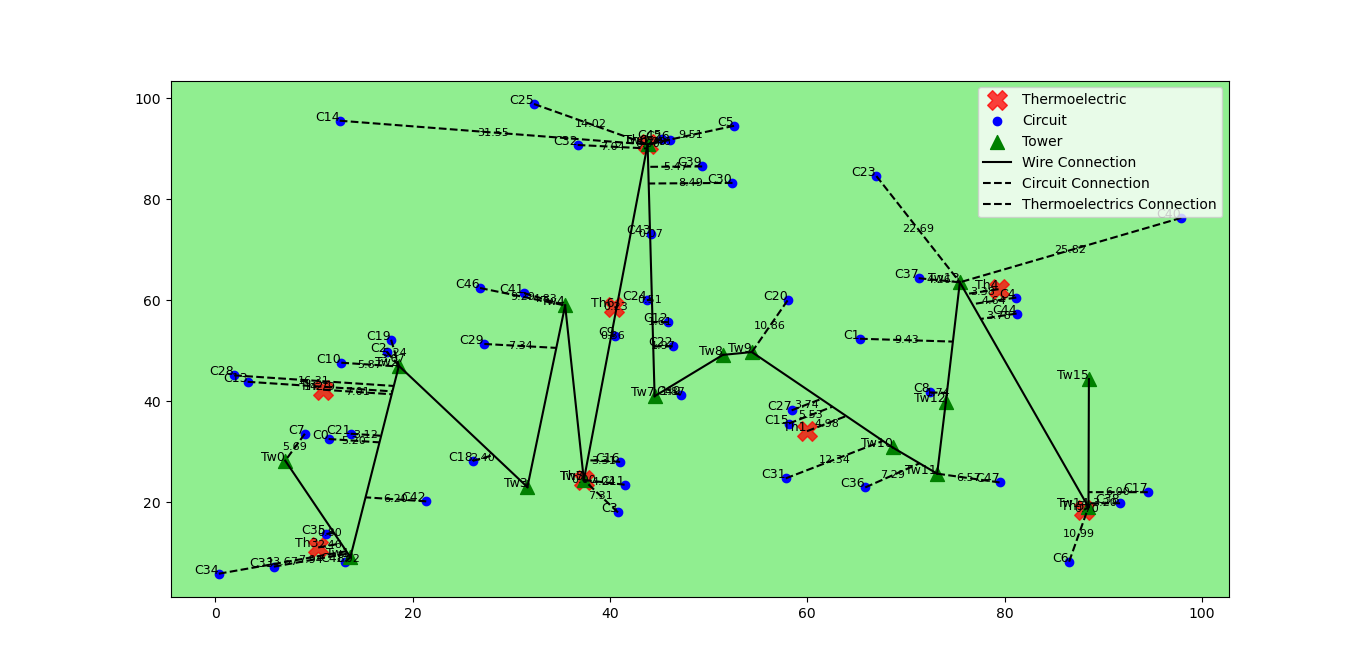
\includegraphics[width=\columnwidth]{assets/map_example.png}
  \caption{Ejemplo de mapa.}
  \label{fig:ejemplo}
\end{figure}

\section{Agentes con Arquitectura BDI}

La arquitectura BDI (Beliefs-Desires-Intentions) en la simulación mediante agentes
les permite modificar su conocimiento del medio o creencias a través del recibimiento
de una percepción, generar nuevas opciones para reformular sus deseos y filtrar las intenciones
que debe tener para llevarlos a cabo, para de esta manera actuar e interactuar para lograr sus objetivos. \cite{book}
En este proyecto fueron utilizados dos tipos de agentes con arquitectura BDI:
\begin{itemize}
  \item \textbf{Agente de Termoeléctrica}: Existe uno en cada Termoeléctrica y sus objetivo es mantenerla funcionando para aportar el mejor rendimiento posible al Sistema Eléctrico.
  \item \textbf{Jefe de la Empresa Eléctrica}: Existe solo uno y se encarga de encontrar y ejecutar la mejor planificación posible de la distribución de energía en dependencia de sus circunstancias en cada momento.
\end{itemize}

\subsection{Agente de Termoeléctrica}
Su percepción se basa en el conocimiento del estado de su 
termoeléctrica y de algunos datos del estado general del 
sistema como la demanda y la oferta del día anterior. 
También puede conocer un tiempo estimado de rotura de las 
piezas de la termoeléctrica, lo cual serviría para planificar 
posibles mantenimientos, su máxima generación posible, su generación actual y
la pérdida de capacidad de generación ante la rotura de una pieza.\\
\textbf{Beliefs}

\begin{itemize}
  \item \textbf{plant\_is\_working}: True si la Planta Termoeléctrica del Agente está funcionando, False en caso contrario.
  \item \textbf{parts\_status}: Una lista de tuplas con 3 elementos, donde el primer elemento es la instancia de la parte, el segundo es True si la parte está funcionando y False en caso contrario, y el tercer elemento indica el tiempo de vida útil estimado restante.
  \item \textbf{broken\_parts}: Una lista de partes que están actualmente rotas.
  \item \textbf{max\_capacity}: La capacidad máxima de la Planta Termoeléctrica.
  \item \textbf{current\_capacity}: La capacidad actual de la Planta Termoeléctrica.
  \item \textbf{power\_output\_reduction\_on\_part\_failure}: Una lista de tuplas donde el primer elemento es la Parte y el segundo es la reducción de producción de energía cuando falla.
  \item \textbf{general\_deficit}: El déficit general del Sistema Eléctrico.
  \item \textbf{general\_demand}: La demanda general del Sistema Eléctrico.
  \item \textbf{general\_offer}: La oferta general del Sistema Eléctrico.
  \item \textbf{all\_desires}: Todos los deseos posibles del Agente.
  \item \textbf{current\_desires}: Los deseos actuales del Agente.
\end{itemize}
\textbf{Desires}
\begin{itemize}
  
  \item \textbf{maintain\_maximum\_power\_output}: Deseo de mantener la máxima producción de energía. (True o False)
  \item \textbf{prevent\_unexpected\_breakdowns}: Deseo de prevenir fallos inesperados. (True o False)
  \item \textbf{minimize\_downtime}: Deseo de minimizar el tiempo de inactividad. (True o False)
  \item \textbf{meet\_energy\_demand}: Deseo de satisfacer la demanda de energía. (True o False)
  \item \textbf{prioritize\_critical\_part\_repair}: Deseo de priorizar la reparación de partes críticas. (True o False)
  \item \textbf{repair\_parts}: Deseo de reparar las partes dañadas. Es una lista de tuplas en la que cada tupla contiene una parte de la planta termoeléctrica y un valor booleano que indica si esa parte necesita ser reparada o no.

\end{itemize}

\textbf{Intentions}

\begin{itemize}
  \item \textbf{increase\_power\_output}: Intención de aumentar la producción de energía
  \item \textbf{operate\_at\_full\_capacity}: Intención de operar a plena capacidad
  \item \textbf{perform\_maintenance\_on\_parts}: Una lista de tuplas donde el lado izquierdo es la Parte y el lado derecho es True si la Parte necesita mantenimiento y False en caso contrario.
  \item \textbf{reduce\_downtime}: Intención de reducir el tiempo de inactividad
  \item \textbf{prioritize\_repair\_of\_critical\_parts}: Intención de priorizar la reparación de partes críticas
  \item \textbf{repair\_parts}: Una lista de tuplas donde el lado izquierdo es una Parte y el lado derecho es True si hay intención de reparar la parte y False en caso contrario

\end{itemize}

\subsection{Jefe de la Empresa Eléctrica}

Su percepción está  dada por una lista de todas las termoeléctricas, todos los circuitos, la matriz de las dictancias entre objetos del mapa, la demanda po bloque, la generación por termoeléctrica, el coeficiente de importancia, industralización y estado de opinión por circuito, un registro de los cortes de electricidad que han ocurrido y los datos generales del sistema como el déficit. \\

\textbf{Beliefs}

\begin{itemize}
    \item thermoelectrics\_id: El identificador único de cada termoeléctrica.
            \item circuits\_id: El identificador único de cada circuito.
            \item generation\_per\_thermoelectric: La electricidad generda por cada termoeléctrica.
            \item distance\_matrix: El costo de transmitir energía de cada termoelétrica a cada circuito.
            \item demand\_per\_block\_in\_circuits: La demanda por hora de cada bloque en cada circuito.
            \item total\_demand\_per\_circuits: La demanda total por hora por cada circuito.
            \item general\_demand: La demanda general del sistema.
            \item general\_offer: La generación total del sistemma.
            \item general\_deficit: El déficit total del sistema.
            \item circuits\_importance: El coeficiente de importanccia de cada circuito.
            \item importance\_per\_block\_in\_circuits: El coeficiente de importancia de cada bloquee.
            \item opinion\_per\_block\_in\_circuits: El estado de opinión de los ciudadanos de cada bloque.
            \item opinion\_per\_circuit: El estado de opinión de los ciudadanos de cada bloque.
            \item industrialization\_per\_circuit: El coeficiente de industrialización de cada circuito.
            \item last\_days\_off\_per\_block\_in\_circuits: El número de días con corte de electricidad por cada bloque.
            \item longest\_sequence\_off\_per\_block\_in\_circuits: El número de días consecutivos con cortes de electricidad por cada bloque.
            \item working\_thermoelectrics\_amount: El número de termoeléctricas que se encuentran funcionando.
            \item thermoelectric\_state: El estado operacional de cada termoeléctrica.
            \item general\_opinion:  El estado de opinió general de los ciudadanos del sistema.
            \item all\_desires: El conjunto de todos los posibles deseos.
            \item current\_desires: El conjunto de deseos actualmente activos.
\end{itemize}

\textbf{Desires}

\begin{itemize}
  \item \textbf{meet\_demand}: Satisfacer la demanda en situaciones de déficit de generación
  \item \textbf{prioritize\_block\_importance}: Priorizar el abastecimiento a los bloques más importantes
  \item \textbf{prioritize\_block\_opinion}: Priorizar el abastecimiento a los bloques con peor opinión ciudadana
  \item \textbf{prioritize\_consecutive\_days\_off}: Priorizar el abastecimiento a los bloques con más días consecutivos sin energía
  \item \textbf{prioritize\_days\_off}: Priorizar el abastecimiento a los bloques que han tenido más cortes de electricidad
\end{itemize}
\textbf{Intentions}

\begin{itemize}
  \item \textbf{meet\_demand}: Intención de satisfacer la demanda incrementando la capacidad actual.
  \item \textbf{prioritize\_block\_importance}: Intención de priorizar bloques con mayor importancia.
  \item \textbf{prioritize\_block\_opinion}: Intención de priorizar bloques basándose en las opiniones de sus ciudadanos.
  \item \textbf{prioritize\_consecutive\_days\_off}: Intención de priorizar los bloques con más días consecutivos con cortes de electricidad.
  \item \textbf{prioritize\_days\_off}: Intención de priorizar los bloques con más días con cortes de electricidad.
\end{itemize}

Este agente tiene la peculiaridad de poseer dinamismo en cuanto a la elección de sus opciones
para generar los \textit{desires}. Ello se logra mediante la comunicación con un \textbf{LLM}, al que se le proporciona una instrucción inicial con una lista de los
posibles \textit{desires} y ciertas condiciones y su tarea es proporcionar la lista de condiciones seleccionadas y la lista de \textit{desires} que considera que deberían ser activados
bajo esas condiciones. De esta forma se logra generar desires de una forma más dinámica y flexible. En próximas secciones se abordará más sobre el \textbf{LLM}.
\section{Algoritmo Genético}

Para que el agente \textbf{Jefe de la Empresa Eléctrica} sea capaz de resolver el problema de búsqueda de decidir una buena planificación
de la dstribución de electricidad se decidió implemnetar un \textbf{Algoritmo Genético}. Para ellos se siguieron los siguientes pasos:
\textbf{inicialización}, \textbf{evaluación}, \textbf{selección}, 
\textbf{cruce (\textit{crossover})}, \textbf{mutación}, y \textbf{repetición a través de 
generaciones}.\\

\textbf{Inicialización}

El algoritmo empieza creando una población 
inicial de soluciones aleatorias (cromosomas), cada una de 
ellas representando una posible asignación de termoeléctricas a bloques. 
El tamaño de la población es definido por el parámetro \textbf{pop\_size}. 
En nuestra población cada cromosoma es una matriz (lista de listas), donde cada fila 
representa el estado de asignación de termoeléctricas a bloques 
en un momento del día (24 horas en total). \\

\textbf{Evaluación}

Cada cromosoma es evaluado usando una función de aptitud (\textit{fitness function}), 
que mide cuán buena es la asignación, teniendo en 
cuenta las intenciones del \textbf{Jefe de la Empresa Eléctrica}. \\
(Describir como se comporta la funcion de fitness). \\
aaaaaaaaaaaaaaaaaaaaaaaaaaaaaaaaaaaaaaaaaaaaaaaaaaaaaaa\\
aaaaaaaaaaaaaaaaaaaaaaaaaaaaaaaaaaaaaaaaaaaaaaaaaaaaaaaaa\\
aaaaaaaaaaaaaaaaaaaaaaaaaaaaaaaaaaaaaaaaaaaaaaaaaaaaaaaaa\\
aaaaaaaaaaaaaaaaaaaaaaaaaaaaaaaaaaa

\textbf{Selección}

Después de evaluar a la población, se seleccionan los mejores 
cromosomas (las soluciones más aptas) para servir de modelos de 
la siguiente generación. \\

\textbf{Cruce}

Se combina la información genética de 
los cromosomas seleccionados (padres) para crear nuevos 
cromosomas (hijos). Este paso introduce diversidad en la 
población y permite que las características de ambos padres se 
transmitan a los hijos. La selección de las parejas a combinar 
se realiza de forma aleatoria. \\

\textbf{Mutación}

Después del cruce, se introduce 
una probabilidad de mutación en los cromosomas para mantener la 
diversidad genética y evitar la convergencia prematura. 
Un cromosoma puede experimentar una pequeña alteración 
(como reasignar una termoeléctrica a un bloque diferente). 
La tasa de mutación controla la frecuencia con 
la que ocurre este proceso. \\


\textbf{Repetición a través de generaciones}

El algoritmo continúa repitiendo 
los pasos de evaluación, selección, cruce y mutación por un 
número definido de generaciones. En cada generación se crea 
una nueva población que reemplaza a la anterior, con la 
esperanza de que las soluciones mejoren con el tiempo. El 
algoritmo compara los cromosomas generados con el mejor 
cromosoma encontrado hasta el momento y lo actualiza si 
encuentra uno con mejor aptitud. Al finalizar el número de 
generaciones, el algoritmo devuelve el mejor cromosoma 
encontrado y su valor de aptitud

\section{Lógica Difusa}

Para evaluar el nivel de satisfacción personal de los ciudadanos de un bloque y con ello generar el estado de opinión,
se utiliza un sistema de \textbf{Lógica Difusa}. Este se encarga de procesar entradas 
imprecisas o subjetivas y generar una salida que representa 
la satisfacción personal. Los factores que influyen en la 
satisfacción personal del ciudadano son los siguientes: 
\begin{itemize}
  \item \textbf{last\_day\_off}: Representa el tiempo transcurrido desde el último día sin electricidad.
  \item \textbf{days\_off\_relation}: Relación entre los días con y sin servicio eléctrico.
  \item \textbf{industrialization}: Refleja el nivel de industrialización del circuito en el que viven los ciudadanos, lo que influye en la necesidad de la energía eléctrica en la prestación de servicios.
  \item \textbf{general\_satisfaction}: Representa la satisfacción general, lo que puede afectar la satisfacción personal.
\end{itemize}

Estas variables se definen de forma difusa en categorías como: reciente, moderado, 
distante, bajísimo, más bajo, bajo, medio y alto. Luego se 
establecen las reglas difusas que determinan cómo la combinación 
de factores de la entrada afectan la satisfacción personal. 
Por ejemplo una regla podría ser que si el último día de 
descanso fue reciente, los días sin servicio son altos, la 
industrialización es baja y la satisfacción general es la más 
baja, entonces la satisfacción personal será baja. Después de 
definir las reglas, se crea un sistema de control difuso que se 
utiliza para realizar simulaciones. Se proporcionan los valores 
de entrada al sistema de simulación, que representan las 
percepciones actuales del ciudadano. Después de proporcionar 
las entradas y aplicar las reglas, el sistema calcula el nivel 
de satisfacción personal. La el atributo \textbf{opinion} de la clase \textbf{Citizen} 
almacena el resultado final, que representa el nivel de satisfacción 
personal del ciudadano basado en las percepciones difusas y 
las reglas.

\section{Modelo Extenso de Lenguaje}

Para agregar dinamismo al comportamiento del agente \textbf{Jefe de la Empresa Eléctrica}
se decidió utilizar un \textbf{Modelo Extenso de Lenguaje} (LLM). Ello se logra proporcionando 
una instrucción al sistema con las especificaciones de lo que se quiere obtener, aclarando 
el formato de la entrada y de la salida. En dicha instrucción se refleja el conjunto total de deseos
del agente, para que al ser proporcionada una lista de condiciones basadas en las percepciones, el modelo decida 
qué deseos deberían ser activados por algún subconjunto de dichas condiciones y de esa forma se genere una nueva regla.
Las consultas al modelo se realizarán en algunos momentos de la simulación.

Se utilizó la API de \textbf{Gemini} de Google, específicamente el modelo \textbf{gemini-1.5-flash}.

\section{Ejecución de la Simulación}

\section{Resultados y Estadísticas}

\section{Conclusiones}


\renewcommand\refname{Referencias}

\begin{thebibliography}{}

  \sloppypar
  \bibitem{parts} Fundación Endesa. (s.f.). Central térmica convencional. Fundación Endesa. \url{https://www.fundacionendesa.org/es/educacion/endesa-educa/recursos/centrales-electricas-convencionales/central-termica-convencional}


  \bibitem{book} García Garrido, L., Martí Orosa \& L., Pérez Sánchez, L. (n.d.) Temas de Simulación. [Publisher not identified]

\end{thebibliography}
    
    

\end{document}
